\documentclass[11pt,a4paper]{article}
\usepackage[utf8]{inputenc}
\usepackage[francais]{babel}
\usepackage[T1]{fontenc}
\usepackage{amsmath}
\usepackage{amsfonts}
\usepackage{amssymb}
\usepackage{makeidx}
\usepackage{graphicx}
%\usepackage{lmodern}
%\usepackage{fourier}
\usepackage[left=2cm,right=2cm,top=2cm,bottom=2cm]{geometry}
\usepackage{titlepic}
\usepackage{color}
\usepackage[table]{xcolor}
%\usepackage{listings}
\usepackage{minted}
\definecolor{darkWhite}{rgb}{0.94,0.94,0.94}
\usepackage[backgroundcolor= darkWhite,frametitle={Code Python}]{mdframed}
\surroundwithmdframed{minted}



%\usepackage{lipsum}
%\usepackage{fancyhdr}

\author{BELHADJI, Yanis ; CAZALS, Laure ; GUNNY, Masoodah ; RODRÍGUEZ CORTÉZ, Carlos Alfonso}
%\title{}



\begin{document}

\begin{titlepage}
    
\includegraphics[scale=0.4]{logo.png}
    \begin{center}
    \vspace*{7cm}
    {\Huge  \textbf{UE 3M101 - }}{\huge \textbf{PROJET}}
    \\
    \vspace{1.5cm}
    \huge \textbf{ONDES}
    \vfill

    {\large  Encadrant : CAZENAVE, Thierry}
    \\~\\
    {\normalsize BELHADJI, Yanis ; CAZALS, Laure ; GUNNY, Masoodah ; RODRÍGUEZ CORTÉZ, Carlos Alfonso}
    \\
    \vspace{1cm}
    {\normalsize Année 2019-2020}
    \end{center}
\end{titlepage}
 
 
\thispagestyle{empty}
\vspace*{\fill}
\renewcommand{\contentsname}{\Huge Sommaire}
\tableofcontents
\vspace{\fill}


\pagebreak
\setcounter{page}{1}

\section{Introduction}
La première équation aux dérivées partielles est apparue pour expliquer le phénomène de vibration d'une corde fixée à ses extrémités, et fut présentée sous la forme suivante par Jean le Rond d'Alembert (1746) :
    \begin{equation} \label{Ondes} 
    \begin{cases} 
    \displaystyle \frac {\partial ^2 u } {\partial t ^2} = \frac {\partial ^2 u } {\partial x ^2}  \quad  \text{pour}\quad t\ge 0, x\in (0,\pi ) \\ u(t, 0)= u (t, \pi )= 0\quad  \text{pour} \quad t\ge 0
    \end{cases} 
    \end{equation} \\
où la fonction $u(t, x)$ représente le déplacement transversal du point $x$ de la corde (considérée tendue) à l'instant $t$ par rapport à sa position d'équilibre. Cette équation correspond au cas où les oscillations sont petites.\\

D'autres équations et systèmes d'équations différentielles ont été proposés pour mieux décrire les phénomènes vibratoires en physique. Ces objets sont d'une grande importance dans certains domaines  comme la mécanique des fluides, l'optique, et même la mécanique quantique.\\

L'objectif de ce projet est de présenter quelques cas d'équations différentielles décrivant des ondes, d'en trouver les solutions au moyen d'un calcul numérique et d'en discuter les particularités, notamment les différents régimes d'oscillation auxquels donnent naissance ces différents systèmes.\\
Nous allons étudier les deux équations ci-dessous :
    \begin{equation} \label{KC} \tag{KC}
    \begin{cases} 
    \displaystyle \frac {\partial ^2 u } {\partial t ^2} =  \Bigl( 1+ \int _0^\pi  \Bigl( \frac {\partial u} {\partial x} \Bigr)^2 \Bigr) \frac {\partial ^2 u } {\partial x ^2} \quad  \text{pour}\quad t\ge 0, x\in (0,\pi ) \\ u(t, 0)= u (t, \pi )= 0\quad  \text{pour} \quad t\ge 0
    \end{cases} 
    \end{equation} 



    \begin{equation} \label{CHW} \tag{S}
    \begin{cases} 
    \displaystyle \frac {\partial ^2 u } {\partial t ^2} = \frac {\partial ^2 u } {\partial x ^2} -  \Bigl( \int _0^\pi u(t,s)^2 ds \Bigr) u \quad  \text{pour}\quad t\ge 0, x\in (0,\pi ) \\ u(t, 0)= u (t, \pi )= 0\quad  \text{pour} \quad t\ge 0
    \end{cases} 
    \end{equation} 
    \\
Le système \eqref{KC} est l'équation de Kirchhoff (ou Kirchhoff-Carrier), et le système \eqref{CHW} est un modèle plus simple qui partage certaines propriétés fondamentales avec \eqref{KC}.\\

\section{Contexte théorique}

Nous cherchons dans un premier temps des solutions dites «modes simples», qui sont de la forme:
\begin{equation} \label{UC2} 
u(t, x) = f(t) \sin ( n x )
\end{equation}  
Cette restriction simplifie notre étude ; Nous obtenons les deux équations équivalentes à \eqref{KC} et \eqref{CHW} respectivement : 
\begin{equation} \label{UC1} 
f '' + n^2  \Bigl( 1+  \frac {\pi } {2} n^2  f^2 \Bigr) f=0
\end{equation} 
 et
\begin{equation} \label{UC3} 
f '' + n^2  f +   \frac {\pi } {2}   f^3 =0
\end{equation} \\

Ces équations possèdent la particularité de pouvoir être mises sous la forme : 
\begin{equation} \label{fSO1} 
U'' + g (U) =0
\end{equation} 

Dans les deux cas, il existe une fonction $G\in C^\infty ( \mathbb{R}^{\ell}, \mathbb{R} )$ telle que
\begin{equation} \label{fSO2} 
g(U) = \nabla G (U), \quad \forall U\in \mathbb{R}^{\ell} .
\end{equation} 
Plus précisément, pour \eqref{UC1} $G (U)=   \frac {n^2} {2} U^2+  \frac {\pi n^4} {8}   U^4 $, et pour \eqref{UC3}   $G(U)=  \frac {n^2} {2} U^2 +   \frac {\pi } {8}   U^4$. 

A son tour, l'équation \eqref{fSO1} peut se mettre sous la forme plus générale
\begin{equation} \label{fCL1} 
V' = \Phi (V) 
\end{equation} 
où $V=V(t) \in \mathbb{R}^N $ et $\Phi : \mathbb{R}^N \to \mathbb{R}^N$ est de classe $C^\infty $. 
Il suffit pour cela de remarquer que \eqref{fSO1} peut s'écrire comme un système
\begin{equation} \label{fSO5} 
\begin{cases} 
U'= W \\ W' = - g( U). 
\end{cases} 
\end{equation} 
Nous posons alors $N= 2 \ell $ et on définit $\Phi : \mathbb{R}^N \to \mathbb{R}^N $ par
\begin{equation} \label{fSO6} 
\Phi \begin{pmatrix} U \\W \end{pmatrix} = \begin{pmatrix} W \\ - g(U) \end{pmatrix} 
\end{equation} 
pour $U, W\in \mathbb{R}^\ell$. 
\\

Nous étendons notre étude aux solutions qui sont des superpositions de modes simples : 
 \begin{equation} 
 u(t,x)= f(t) \sin ( j x) + g (t) \sin ( k x )
 \end{equation} \\
 Pour le système~\eqref{KC}, il est commode de poser
\begin{equation} \label{KC2} 
f (t)= \frac {1} {j}  \phi   ( j t )  \sqrt{\frac {2} {\pi }} , \quad g (t) = \frac {1} {j}  \psi   ( j t )  \sqrt{\frac {2} {\pi }} , \quad \mu =  \Bigl( \frac {k} {j} \Bigr)^2
\end{equation} 
de façon que le système~\eqref{KC} devienne
 \begin{equation} \label{KC3} 
\begin{cases} 
\phi  '' + \phi  +    ( \phi ^2 + \mu  \psi ^2 ) \phi  =0 \\
\psi  '' + \mu \psi  +  \mu ( \phi ^2 + \mu  \psi ^2 ) \psi  =0 
\end{cases} 
\end{equation} 
Notons qu'en posant $ \varphi  = \mu ^{\frac {1} {2}} \psi $, le système~\eqref{KC3} s'écrit
 \begin{equation} \label{KC4} 
\begin{cases} 
\phi  '' + \phi  +    ( \phi ^2 +   \varphi ^2 ) \phi  =0 \\
\varphi  '' + \mu  \varphi +  \mu ( \phi ^2 +   \varphi ^2 )  \varphi =0 
\end{cases} 
\end{equation} 
Pour le système~\eqref{CHW}, nous posons
\begin{equation} \label{CHW2} 
f (t)= j \phi   ( j t ) \sqrt{\frac {2} {\pi }} , \quad g (t) = j \psi   ( j t ) \sqrt{\frac {2} {\pi }} , \quad \mu =  \Bigl( \frac {k} {j} \Bigr)^2
\end{equation} 
de façon que le système~\eqref{CHW2} devienne
 \begin{equation} \label{CHW3} 
\begin{cases} 
\phi  '' + \phi  +    ( \phi ^2 + \psi ^2 ) \phi  =0 \\
\psi  '' + \mu \psi  +  ( \phi ^2 + \psi ^2 ) \psi  =0 
\end{cases} 
\end{equation} 
En posant $\phi = U_{1}, \psi = U_{2}, \phi ' = W_{1}, \psi ' = W_{2}$, nous réécrivons les deux systèmes \eqref{KC4} et \eqref{CHW3} sous la forme \eqref{fSO6} . Nous avons alors le système suivant :
\begin{equation} \label{fSO6} 
\Phi \begin{pmatrix} U_{1}\\ U_{2} \\W_{1} \\ W_{2}  \end{pmatrix} = \begin{pmatrix} W_{1}\\ W_{2} \\ - g(U_{1})\\ -g(U_{2}) \end{pmatrix} 
\end{equation} 

\pagebreak
\section{Étude du système \eqref{CHW}}

En utilisant le langage Python, nous allons étudier le système \eqref{CHW3} dont les solutions sont les modes simples du système \eqref{CHW}.
En particulier nous allons coder la fonction \eqref{fSO6} correspondante pour résoudre numériquement ce système.

    \subsection{Résolution numérique}
    
Nous commençons par définir notre fonction \textbf{F\_15} dans un fichier dédié que nous appelons \textbf{F\_ode}. Nous utilisons notamment la bibliothèque \textbf{\textit{numpy}} avec l'alias \textbf{\textit{np}}.\\ 

\begin{minted}[linenos]{python}
import numpy as np
"""
Définition de la fonction qui renvoie la dérivée de phi,psi,phi' et psi' 
pour le système 15 avec la syntaxe correspondant à odeint.
"""

def F_15(tab,t,M):
    phi,psi,vphi,vpsi = tab
    du = np.array([vphi, vpsi, - phi - (phi**2 +psi**2)*phi, 
         -M*psi -(phi**2 +psi**2)*psi])
    return du

\end{minted} 

Cette fonction prend en argument : 
\begin{itemize}
\item un tableau "tab", contenant les valeurs des conditions initiales pour $(\phi, \psi, \phi',\psi')$;
\item un tableau "t", de N valeurs régulièrement espacées sur l'intervalle de temps considéré que nous définirons par la suite;
\item un paramètre "M", qui correspond à $\mu$ dans notre système. 
\end{itemize}
Elle renvoie en sortie un tableau de valeurs des dérivées du tableau d'entrée c'est à dire $(\phi', \psi', \phi'',\psi'')$. Nous avons donc bien une fonction de la forme \eqref{fSO6}.
Cette fonction nous servira d'argument dans la fonction \textbf{\textit{odeint}} de la bibliothèque \textit{\textbf{scipy.integrate}} qui permet de résoudre numériquement des systèmes d'équations différentielles ordinaires.\\
Nous nous plaçons maintenant dans un fichier séparé et nous utilisons donc la fonction \textit{\textbf{odeint}} pour résoudre le système :\\


\begin{minted}[linenos]{python}
import numpy as np
import matplotlib.pyplot as plt
import matplotlib.gridspec as gridspec
from scipy.integrate import odeint
from F_ode import F_15, test15 
"""On a fait appel ici aux fonctions concernant le système (15) définies 
dans le fichier F_ode"""

#Paramètres:
    M = 2 #mu
    #Intervalle de temps:
        ti = 0
        tf = 30
        N = 10000  #Nombre de pas
    t_ode = np.linspace(ti,tf,N) 
#Conditions initiales:
C0 = np.array([np.sqrt(2),0,15,10])

#Résolution:
solu = odeint(F_33,C0,t_ode, args = (M,))
rsolu = solu[:,[0,1]] #On récupère seulement les deux premières colonnes (Phi,Psi)


\end{minted}

Nous avons à disposition dans le tableau \textit{solu} N valeurs de $\phi$, $\psi$, $\phi'$ et $\psi'$ en fonction du temps qui vont nous permettre de représenter graphiquement les solutions. Nous nous restreignons cependant au tableau \textit{rsolu} qui correspond aux deux premières colonnes de \textit{solu}, soient les valeurs de $\phi$ et $\psi$ qui nous intéressent pour les tracés.

Pour tracer les courbes recherchées, nous utilisons dans la suite du code la bibliothèque \\ \textbf{\textit{matplotlib.pyplot}} avec l'alias \textbf{\textit{plt}} :\\

\begin{minted}[linenos,firstnumber=last]{python} 
#Représentation des solutions :
fig = plt.figure(1, figsize = [9,7], constrained_layout=True)
plt.clf()

#Mise en forme
plt.axis('off')
plt.title("""Solution du système (33) \n 
          Paramètres : ($\phi_0$,$\psi_0$,$\phi_0'$,$\psi_0'$) = ({},{},{},{})\n 
          $\mu$ = {} , t = {} \n""" .format(C0[0],C0[1],C0[2],C0[3],M1,tf))

gs = gridspec.GridSpec(3, 2)  #Mise en page pour la disposition des subplots 

#Tracé de phi en fonction de t:
ax1 = fig.add_subplot(gs[0,0])
plt.title("$\phi = f(t)$", fontsize = 9)
plt.plot(t_ode,rsolu[:,0],'b-',linewidth= 0.3) 

#Tracé de psi en fonction de t:
ax2 = fig.add_subplot(gs[0,1])
plt.title("$\psi = f(t)$", fontsize = 9)
plt.plot(t_ode,rsolu[:,1],'b-',linewidth= 0.3) 

#Tracé de psi en fonction de phi:
ax3 = fig.add_subplot(gs[1:3,:])
plt.title("\n$\psi = f(\phi)$", y=-0.1)

ax3.spines['left'].set_position('zero')      #Positionnement de axes au centre
ax3.spines['bottom'].set_position('zero')

ax3.spines['right'].set_color('none')
ax3.spines['top'].set_color('none')      #Suppression des axes inutiles

plt.xticks([])      #Suppression des graduations
plt.yticks([])  

plt.plot(rsolu[:,0],rsolu[:,1],'b-',linewidth= 0.3) 
plt.show()

\end{minted}

Dans cette partie du code, nous utilisons donc les valeurs de $\phi$ et $\psi$ obtenues en fonction du temps et nous traçons trois graphiques sur la même figure:
\vspace{0.2cm}
\begin{itemize}
\item $\phi$ en fonction du temps, \textit{t\_ode};
\item $\psi$ en fonction du temps, \textit{t\_ode};
\item $\psi$ en fonction de $\phi$, tel que présenté dans notre document de référence.
\end{itemize}
\vspace{0.2cm}
    Chacune de ces représentations est tracée sur un "sous-graphique" appelé \textit{\textbf{subplot}}. Pour cela, nous utilisons la commande \textit{\textbf{plt.plot(x,y)}} qui permet de tracer des points sur le graphique, en indiquant l'abscisse et l'ordonnée souhaitées ainsi que des commandes de mise en forme.
Les \textit{\textbf{subplots}} sont ensuite arrangés sur une même figure en utilisant plusieurs options de mise en page pour améliorer la lisibilité.

Nous obtenons par exemple une figure comme celle-ci :\\
 \begin{center}
 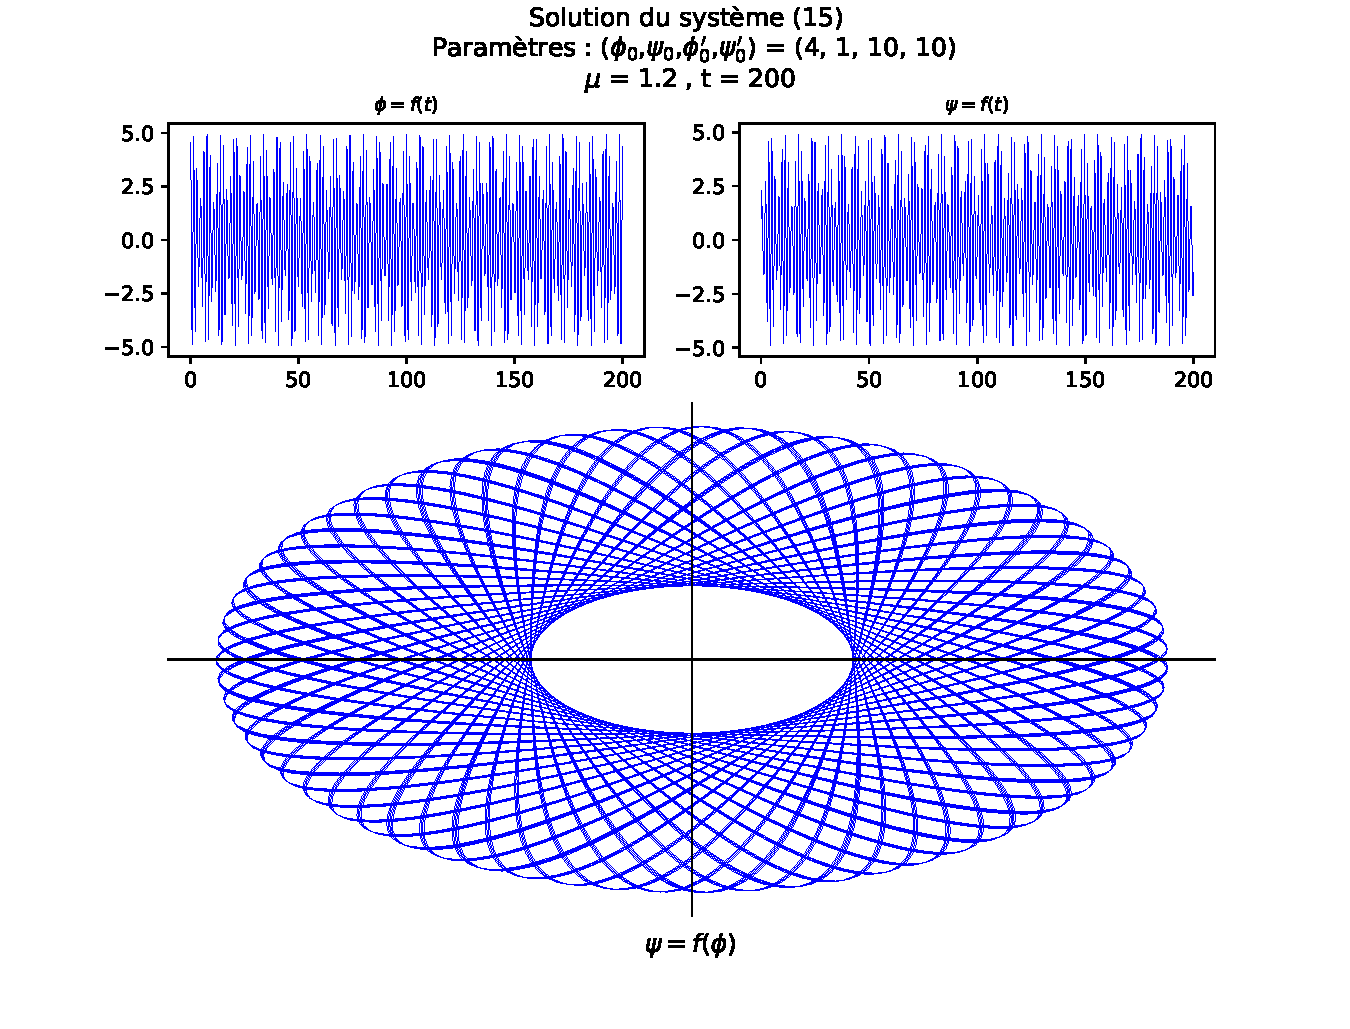
\includegraphics[scale=0.7]{REGIME1_ODE33.pdf}
 \end{center}

%%Notes:
    % A TERMINER : ->en faisant varier les conditions initiales on retrouve bien deux régimes comme dans le poly..., + images de chacun des régimes. +Changer le numéro des système sur les images.
    
    %Partie solution exceptionnelle: méthode par dichotomie entre les deux régimes, image de la "singularité" + explication avec la fin du poly = code de la fonction test_15 et exemple de valeur...
    %Dans le contexte thélrique: ajout des systèmes 27 et 28 du poly avec le raisonnement qu'il y a avant?

    \subsection{Phénomène de transfert d'énergie (solutions exceptionnelles)}
\section{Résolution de l'équation de Kirchhoff (système \eqref{KC})}
    \subsection{Simplification de l'équation}
    \subsection{Résolution numérique}
    \subsection{Phénomène de transfert d'énergie (solutions exceptionnelles)}

\section{Solution à un système inédit}


\end{document}


